%!TEX root = ../template.tex
%%%%%%%%%%%%%%%%%%%%%%%%%%%%%%%%%%%%%%%%%%%%%%%%%%%%%%%%%%%%%%%%%%%
%% chapter4.tex
%% NOVA thesis document file
%%
%% Chapter with introduction
%%%%%%%%%%%%%%%%%%%%%%%%%%%%%%%%%%%%%%%%%%%%%%%%%%%%%%%%%%%%%%%%%%%

\typeout{NT FILE chapter4.tex}%

\chapter{Spectra simulation}
 
This chapter is the culmination of all the work performed on this thesis. Synthetic theoretical spectra will be computed using the calculated parameters from chapters~\ref{cha:atom_calc} and~\ref{cha:parameters}. For the simulation of the resonant effect, a new approximate method for estimating photoexcitation cross-sections will be developed.

\section{Theoretical line shapes}

Even though an atomic state transitions possess well-defined energy values, as calculated in chapter~\ref{cha:atom_calc}, it is now also clear that these transitions also have an energetic uncertainty to them, given by the sum of the energy widths of the initial and final levels (equation~\eqref{eq:trans_width}). The theoretical emission shape is given by a Lorentzian profile, centered around the emission energy, $E_{i,f}$, with a FWHM of $\Gamma_{i,f}$ and an amplitude of $I_{i,f}$:

\begin{equation}
    L\equiv L\qty(E-E_{i,f},\Gamma_{i,f},I_{i,f})=\frac{I_{i,f}}{2\pi}\frac{\Gamma_{i,f}}{\qty(E-E_{i,f})^2+\qty(\Gamma_{i,f}/2)^2},
    \label{eq:Lorentzian}
\end{equation}

This profile, however, would only be valid for the emission of radiation by stationary atoms (with no thermal distribution) and does not account for the detection of said radiation and interactions it may have with the experimental apparatus, with these last considerations being nondeterministic, but stochastic in nature. To account for this, a new broadening should be considered.

A common way to tackle this problem is to compute the convolution of the theoretical shape from equation~\eqref{eq:Lorentzian} with the Gaussian profile from equation~\eqref{eq:Gaussian}. 

\begin{equation}
    G\equiv G\qty(E,\sigma)=\frac{1}{\sigma\sqrt{2\pi}}\exp(-\frac{E^2}{2\sigma^2}),
    \label{eq:Gaussian}
\end{equation}

The $\sigma$ parameter should account for Doppler shifts caused by thermal distributions, stochastic effects in the experimental setup and the radiation detection system's resolution. This operation results in a specific type of profile also known as Voigt:

\begin{equation}
    V\equiv V\qty(E-E_{i,f},\Gamma_{i,f},\sigma,I_{i,f})=\int_{-\infty}^{\infty} L\cdot G\dd{E},
\end{equation}

Due to the complexity of the convolution operation, there is no simple analytical expression for obtaining values from the Voigt distribution. They can, however, be computed by taking the Real part of the Faddeeva function, $w(z)$:

\begin{equation}
    V\qty(z)= \frac{\Re{w\qty(z)}}{\sigma\sqrt{2\pi}},\quad z=\frac{E-E_{i,f} + i\Gamma_{i,f}}{\sigma\sqrt{2}},
\end{equation}

In Figure~\ref{fig:Lor_Voigt}, the theoretical $K_\alpha$ spectrum for ionized Copper, using the $N_i=1$ approximation, previously mentioned in section~\ref{sec:trans_int}, is displayed for both when only accounting for emission, and for when considering an experimental resolution of $2\ \si{\electronvolt}$.

\begin{figure}[h!]
    \centering
    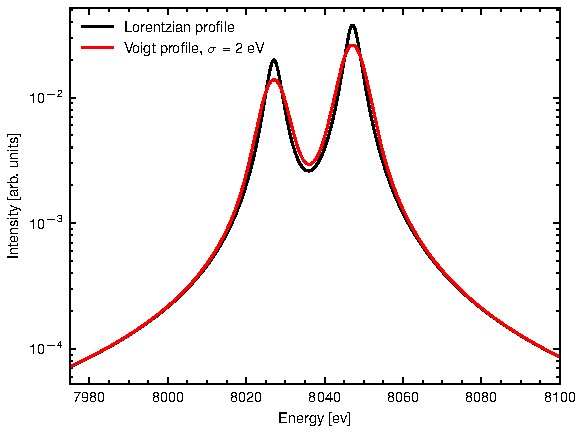
\includegraphics[width=.6\linewidth]{Chapters/Figures/Chapter4/K_lorentz_voigt.pdf}
    \caption{Comparison of a Lorentzian and Voigt profile for Copper's characteristic $K_{\alpha}$ transitions. The red line is the obtained result after convolution the black line with a $\sigma=2\ \si{\electronvolt}$ Gaussian profile.}\label{fig:Lor_Voigt}
\end{figure}


\section{Computing the photoexcitation effect}


The final step needed  in order to simulate the theoretical spectra is that of calculating the scaling factor $N_i$ as a function of the energy of the incident beam.

\subsection{The beam profile}


The objective for this thesis is that of simulating the effect an x-ray beam coming from a synchrotron line with energies close to that of Copper's K-shell ionization  threshold has on the measured x-ray emission spectrum. The incident synchrotron radiation, through the usage of wigglers and undulators can reach a near monochromatic distribution, with energy spreads on the scale of only a few hundred $\si{\milli\electronvolt}$.


From this point forward, a Gaussian profile will be considered for the incident beam. This profile has a tunable energy, in order to survey the whole near-ionization threshold region, and a broadening parameter $\sigma=0.5\ \si{\electronvolt}$.

\subsection{Simulating the resonance}

It is now necessary to calculate the $N_i$ parameter as to account for both the beam profile and the resonance. For an accurate spectra simulation, this value should be that of the photoexcitation cross-section. This, however, is simply not easy to calculate.\todo{meter esta parte melhor} While \gls{MCDFGME} is able to calculate photionization cross-sections, it is not for the photoexcitation case. Experimental data was also not found, but that would go against the \textit{ab-initio} objective of this thesis. A good approach would be to perform R-Matrix calculations \todo{cite here}, but due to their complexity, it was not possible to achieve this at this stage.

In order to solve this problem, assumptions had to be made. First, steady state was assumed, as well that every Cu atom could only be found in ground state before beam-interaction. Second, for every given transition, three states were assumed: the initial ground state, the intermediate excited state, and the final post-relaxation state.

In order to estimate a scaling factor for the population of the intermediate state, it was assumed that, for a given beam energy distribution, the rate of excitation from the ground state to the excited state would be proportional to that of the direct decay from the excited to ground state, since the mediation interaction is the same for both of them, only on an inverse order. Both processes occur with a photon absorbed/emitted  from the system and an electron changing orbital.

Since for the purpose of  state population only the decay from the excited state to the ground state was accounted for, the full width of the transition is only composed by that single partial width, since there is only one decay channel. In order to compute the parameter $N_i$, the overlap of the beam profile and a Lorentzian profile with width equal to that of the transition and with an amplitude equal to the rate was taken:

\begin{equation}
    N_i =R_{exc} \int_{-\infty}^\infty G\qty(E-E_{beam},0.5\ \si{\electronvolt})\cdot L(E-E_{exc},\Gamma_{exc}) \dd{E},
\end{equation}

This way it is ensured the resonance peak occurs at the excitation energy and takes into account the beam energetic distribution.

Taking into account every calculated excited state, Figure~\ref{fig:absorption} contains every Lorentzian contribution. This resonant spectrum could be somewhat proportional to the excitation component of Copper's absorption spectrum. 


\begin{figure}[h!]
    \centering
    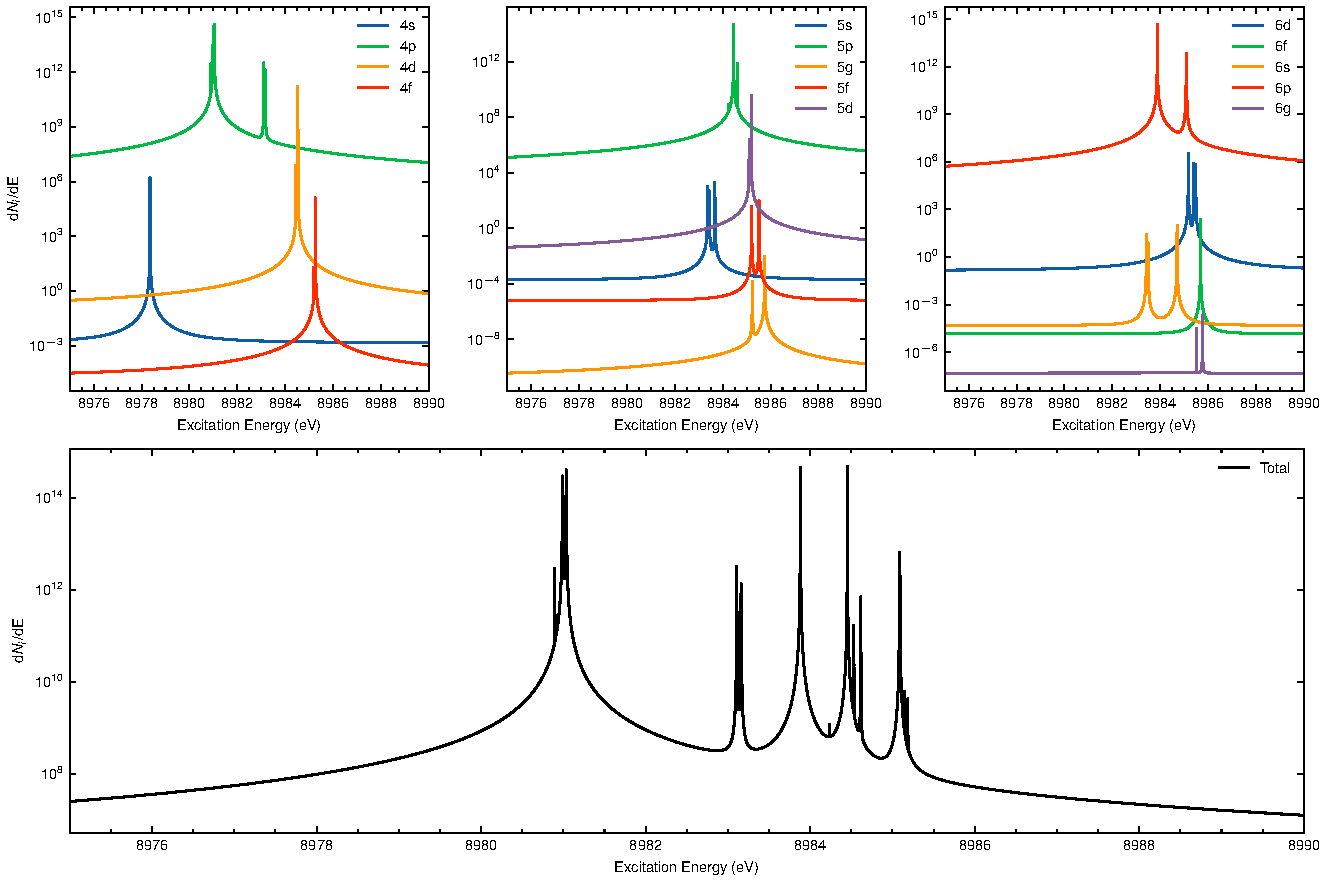
\includegraphics[width=\linewidth]{Chapters/Figures/Chapter4/absorption.pdf}
    \caption{Differential scaling parameter accounting for every excitation contribution. The legend indicates the orbital the electron was excited to.}\label{fig:absorption}
\end{figure}

From Figure~\ref{fig:absorption}, there is something quite notorious. While for most excited states, the absorption energies related to K-shell excitation can be found close together, in the case of the excitation to orbital $4p$, two levels converged to an energy value diverging from the others by around $3\ \si{\electronvolt}$. While this could have arisen from a numerical convergence problem, all convergence parameters were confirmed and other more complex methods employed, with no change in the level energy. This energy difference will have a great impact in the simulated spectrum, since this excitation is the one with the highest probability.




\section{Computing the photoionization effect}

It is now necessary to account for the effects that ionized Copper has on the spectrum, all while finding a way to calculate $N_i$ that is also compatible with the photoexcited case.


Assuming ground state Copper as a starting point, following the ionization of the K shell, two levels are possible: one where the 1s and the 4s electron's spins counter-align, resulting in a $J$ value of 0 and multiplicity 1, and one where they align, resulting in $J=1$ and a multiplicity of 3. The ionization energy can be calculated for both level possibilities by the energetic difference between the levels, resulting in a theoretical value of $8986.02502\ \si{\electronvolt}$ for the singlet and $8985.93363\ \si{\electronvolt}$. It should be noted that the theoretical values are shifted by more than $5\ \si{\electronvolt}$ from most values present for solid-state Copper in the standard x-ray databases, such as xraylib's of $8978.9\ \si{\electronvolt}$~\cite{SCHOONJANS2011776}, and NIST's $ 8 980.476(20) \ \si{\electronvolt}$~\cite{NIST_database}. It is, however, quite similar to the K-edge values for Vaporized Copper, also present in NIST's database $8 987.89(50)\ \si{\electronvolt}$~\cite{NIST_database}. This shift is due to solid-state interactions between the Copper atoms displaying crystalline patterns \todo{Verificar isto} resulting in a decrease in the binding energy.


The photoionization cross-sections were obtained using the \gls{MCDFGME} code,  with the same settings of orthogonality enforcing and no relaxation allowed used for auger transitions for energies from the ionization threshold up to ????\todo{insert later}. Figure ?? displays the obtained results. An independent \gls{MPI} script was developed for faster calculations for a large set of photon energies.

\missingfigure{Meter secções eficazes.Mencionar porque esta em OS (ou meter as duas escalas na figura)}

From the zoom-in view on the previous figure, it is apparent that the cross-section are not accurate for near-ionization energies, as can be seen by the slow rise and oscillatory behaviors. This is an artifact of the calculation method and these values do not display the true nature of the photoionization effect. In order to properly estimate them, a 3-exponential fit was performed for both curves, for higher energies ($10\ \si{\kilo\electronvolt}$), and values were extrapolated for the near-ionization threshold, with a sudden drop to 0 for values lower than the theoretical ionization energy.

\todo{meter aqui valores}

While it was possible to calculate the proper cross-section values, the $N_i$ parameter needed compatibility to the way it was computed in the photoexcited state, so the correlation between the Oscillator Strength and Rate needed was needed.


On the case of radiative transitions, for the electric components, besides yielding the rate value, \gls{MCDFGME} also outputs the correspondent value for the Oscillator Strength. A proportionality was found between these two parameters, the emitted photon energy, and the ratio between the initial and final state multiplicities.

\todo{meter a equação}

It is now possible to convert the photoionization cross-sections into something that is rate normalized so that the overlap can be calculated with the beam profile and the parameter $N_i$ computed. In a similar but inverse fashion, the photoexcitation cross-sections, can be calculated and are present in Annex~??.


\section{The synthetic spectrum}

The energy of the beam profile used for simulation was tuned as to survey the whole pre-excitation region up to post K-shell ionization. From an initial beam energy of $8970\ \si{\electronvolt}$ up to a final of $8995\ \si{\electronvolt}$, in steps of $0.01\ \si{\electronvolt}$, the spectra were simulated taking into account the whole set of contributions. As expected, for the excitations, the diagram transitions for 4p-excited Copper have the greatest impact on the spectrum. This is due to it being the $ns\rightarrow n' p$ excitation to the lowest possible $n'$ value.\todo{Justifica melhor isto} These are followed by other $n'p$-excited states, with the spectral intensity decreasing by an order of magnitude for each consequent $n'$. The spectral 2D plots, containing the x-ray emissions as a function of beam energy for each component can be found in Annex~??, while the full spectrum is present in Figure~??. Due to the previously mentioned energy divergence for some $4p$ excited levels, two distinct resonant areas will appear on the spectrum for this contribution.

\begin{figure}[h!]
    \centering
    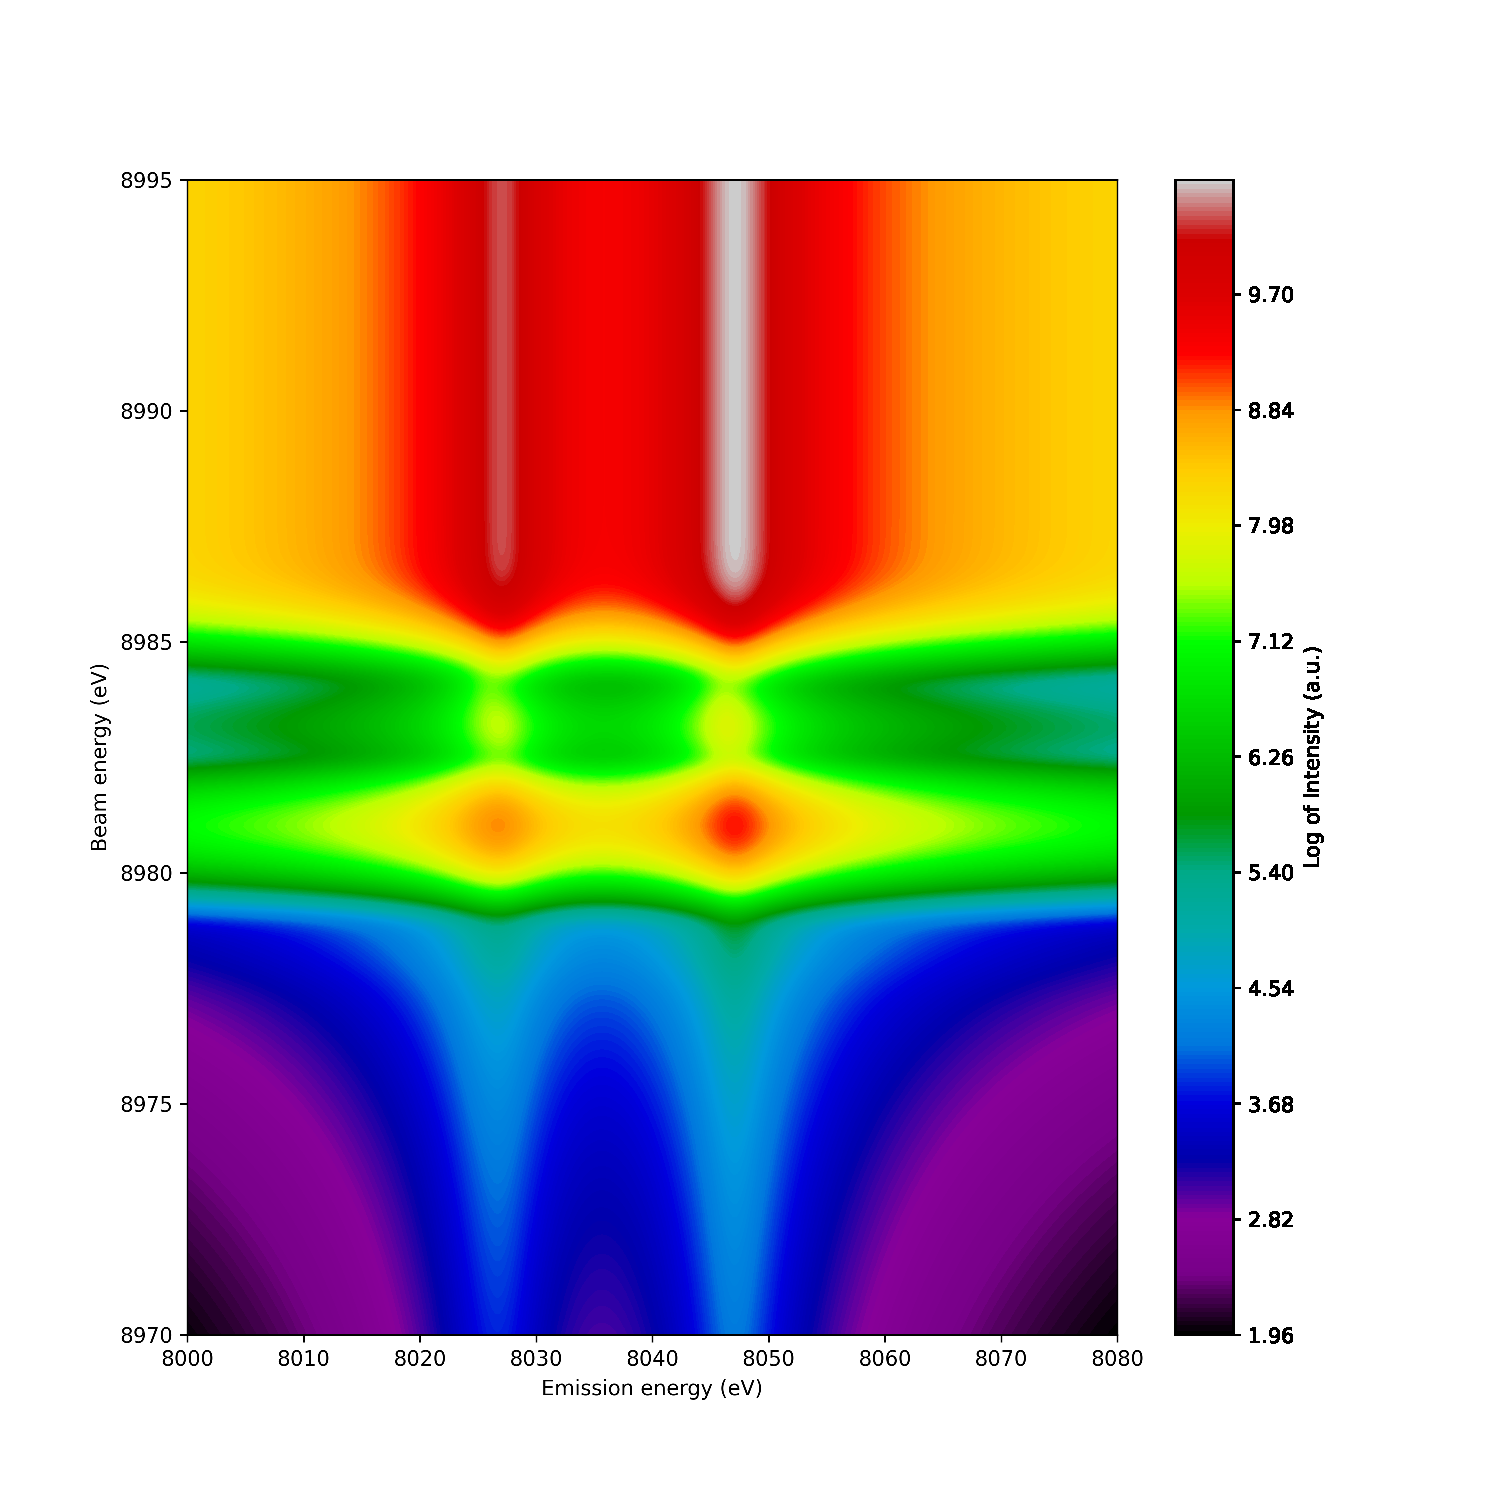
\includegraphics[width=.7\linewidth]{Chapters/Figures/Chapter4/all_log.pdf}
\end{figure}

From these view, it is quite obvious the presence of three high-intensity regions. Both lower energy ones are $4p$-excitation dominated, while the high energy one, where a clear plateau region is observed is due to the photoionization. As expected, this last component would be the dominant one once the threshold has been reached. In the next chapter, the effect other excited states have on the emission energy will be further explored as to be more apparent.


\section{Photoabsorption cross-section}
Not accounting for dispersion.